\subsection{Psf\-Stars  Class Reference}
\label{class_psfstars}\index{PsfStars@{Psf\-Stars}}
a class to select PSF stars from different ways. 


{\tt \#include $<$daophotpsf.h$>$}

Inheritance diagram for Psf\-Stars::\begin{figure}[H]
\begin{center}
\leavevmode
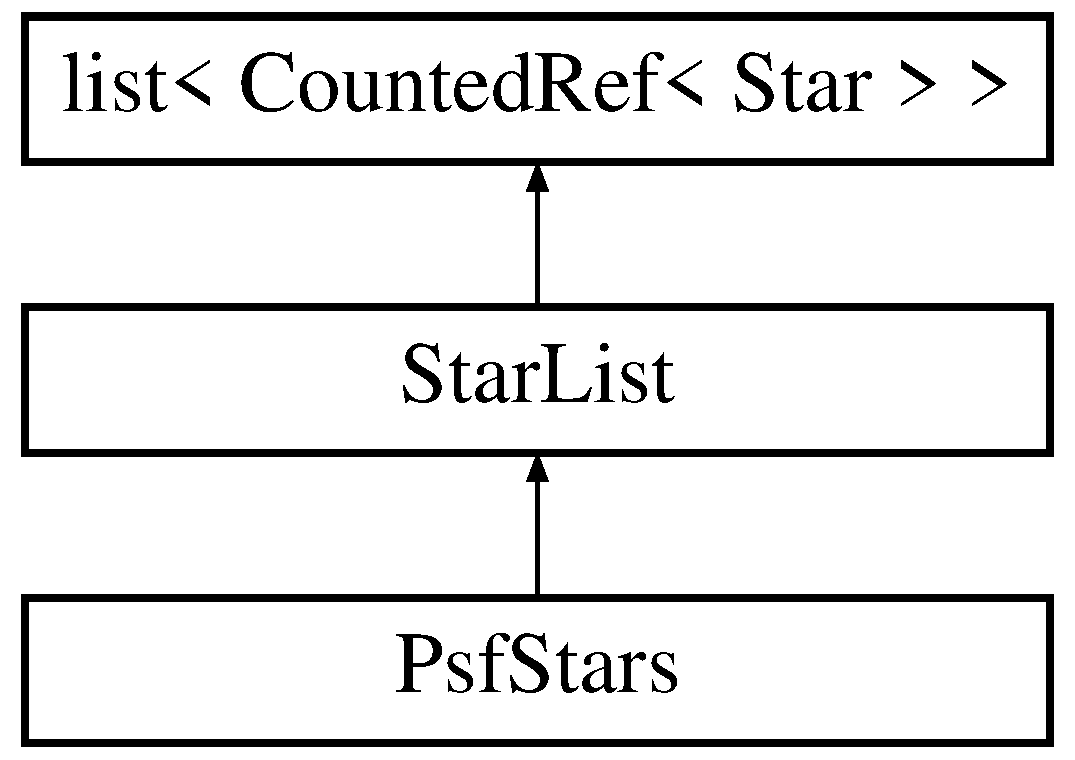
\includegraphics[height=3cm]{class_psfstars}
\end{center}
\end{figure}
\subsubsection*{Public Methods}
\begin{CompactItemize}
\item 
\index{PsfStars@{PsfStars}!PsfStars@{Psf\-Stars}}\index{PsfStars@{PsfStars}!PsfStars@{Psf\-Stars}}
{\bf Psf\-Stars} (const {\bf Reduced\-Image} \&Rim)\label{class_psfstars_a0}

\begin{CompactList}\small\item\em just reads in the decent objects from a {\bf Reduced\-Image} {\rm (p.\,\pageref{class_reducedimage})}.\item\end{CompactList}\item 
\index{~PsfStars@{$\sim$PsfStars}!PsfStars@{Psf\-Stars}}\index{PsfStars@{PsfStars}!~PsfStars@{$\sim$Psf\-Stars}}
{\bf $\sim$Psf\-Stars} ()\label{class_psfstars_a1}

\item 
\index{FilterNei@{FilterNei}!PsfStars@{Psf\-Stars}}\index{PsfStars@{PsfStars}!FilterNei@{Filter\-Nei}}
size\_\-t {\bf Filter\-Nei} ()\label{class_psfstars_a2}

\begin{CompactList}\small\item\em removes the stars with bad flags on the neighbor file created during PSF building.\item\end{CompactList}\item 
\index{FilterAls@{FilterAls}!PsfStars@{Psf\-Stars}}\index{PsfStars@{PsfStars}!FilterAls@{Filter\-Als}}
size\_\-t {\bf Filter\-Als} (const double Chi\-Max=3.0, const double Sharp\-Min=-0.5, const double Sharp\-Max=0.5)\label{class_psfstars_a3}

\begin{CompactList}\small\item\em removes the stars from the file created by ALLSTAR, given some cuts.\item\end{CompactList}\item 
\index{FilterCond@{FilterCond}!PsfStars@{Psf\-Stars}}\index{PsfStars@{PsfStars}!FilterCond@{Filter\-Cond}}
size\_\-t {\bf Filter\-Cond} (const Psf\-Conditions \&Cond)\label{class_psfstars_a4}

\begin{CompactList}\small\item\em removes the stars which do not verify the conditions Cond.\item\end{CompactList}\item 
\index{FilterMultiIm@{FilterMultiIm}!PsfStars@{Psf\-Stars}}\index{PsfStars@{PsfStars}!FilterMultiIm@{Filter\-Multi\-Im}}
size\_\-t {\bf Filter\-Multi\-Im} (const Reduced\-Image\-List \&Rim\-List, const {\bf Reduced\-Image} $\ast$ref, const double Max\-Dist=2)\label{class_psfstars_a5}

\begin{CompactList}\small\item\em keeps the stars in the set of images in Rim\-List.\item\end{CompactList}\end{CompactItemize}


\subsubsection{Detailed Description}
a class to select PSF stars from different ways.



The documentation for this class was generated from the following file:\begin{CompactItemize}
\item 
{\bf daophotpsf.h}\end{CompactItemize}
